\subsubsection{UC6 - Ripristina sessione}
\begin{figure}[h]
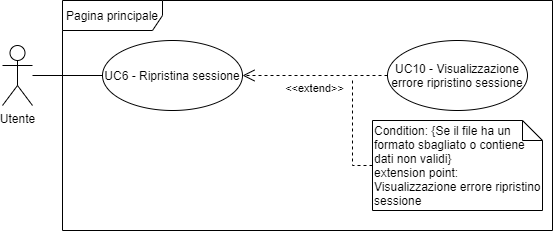
\includegraphics[width=\linewidth]{section/Images/UC6.png}
\centering
\caption{UC6 - Ripristina sessione}
\end{figure}
\begin{itemize}
	\item \textbf{Attore primario}: Utente.
	\item \textbf{Precondizioni}: L'utente è in possesso di un file JSON ottenuto dal salvataggio della sessione [UC5].
	\item \textbf{Postcondizioni}: Viene visualizzato un messaggio che avvisa l'utente del corretto ripristino della sessione. Viene ripristinata la sessione salvata nel file.
	\item \textbf{Scenario principale}:
		\begin{enumerate}
			\item L'utente accede al sistema;
			\item L'utente seleziona la funzionalità "ripristina sessione";
			\item L'utente seleziona il file da caricare.
		\end{enumerate}
	\item \textbf{Estensioni}:
	\begin{enumerate}[(a)]
		\item Nel caso in cui il file abbia un formato sbagliato o contiene dati non validi:
		\begin{enumerate}[1.]
			\item la sessione non viene ripristinata;
			\item viene visualizzato un errore esplicativo [UC10].
		\end{enumerate}
	\end{enumerate}
\end{itemize}